%%%%%%%%%%%%%%%%%%%%%%%%%%%%%%%%%%%%%%%%%%%%%%%%%%%%%%%%%%%%%%%
% JOURNAL INSTRUCTIONS
% This section may be divided by subheadings and should contain sufficient detail so that when read in conjunction with cited references, all procedures can be repeated. For experiments reporting results on animal or human subject research, an ethics approval statement should be included in this section (for further information, see the Bioethics section.)
%%%%%%%%%%%%%%%%%%%%%%%%%%%%%%%%%%%%%%%%%%%%%%%%%%%%%%%%%%%%%%%

% TODOS
% - work in world grid size!

\section{Materials and Methods}

\subsection{The Avida Digital Evolution Platform}

% We conducted our study using the Avida Digital Evolution Platform \citep{ofria_avida:_2009}. 
% Avida provides a computational study system where populations of digital organisms undergo Darwinian evolution, allowing researchers to test hypotheses that would be difficult or impossible to address in natural systems.

% - Define digital organisms -
Avida is a study system wherein self-replicating computer programs (digital organisms) compete for space on a finite toroidal grid \citep{ofria_avida:_2009}.
% Self-replication, however, is imperfect such that organisms mutate randomly and evolve. 
% in a well mixed population(?)
Each digital organism is defined by a linear sequence of program instructions (its genome) and a set of virtual hardware components used to interpret and express those instructions [Figure?].
% Avida tracks each organism as it expresses its genome in a given environment in order to measure that organism's phenotype.
Genomes are expressed sequentially except when the execution of one instruction deterministically changes which instruction should be executed next (e.g., a `jump' instruction). 
Genomes are built using an instruction set that is both robust and Turing Complete [cite]; that is, any ordering of instructions is syntactically valid (though not necessarily meaningful), and genomes are able to represent any computable function (though not necessarily in an efficient manner).
The instruction set includes operations for basic computations, flow control (e.g., conditional logic and looping), input, output, and self-replication.
% @AML: Outsource the next sentence to a figure!
% The virtual hardware set includes components such as a central processing unit (CPU) for executing instructions, registers to store values, buffers for inputs and outputs, and memory stacks \citep{ofria_avida:_2009}.

% - define reproduction & mutation -
Organisms in Avida reproduce asexually by copying their genome instruction-by-instruction and then dividing. 
% However, these operations can be configured to be erroneous, potentially resulting in mutated offspring.
However, copy operations are imperfect and can result in single-instruction substitution mutations in an offspring's genome. 
For this work, we configured copy operations to err at a rate of one expected mutation for every 400 instructions copied (i.e, a per-instruction error rate of 0.0025).
% at a per-instruction rate of 0.0025 (i.e., one mutation expected for every 400 instructions copied).
We held individual genomes at a fixed length of 100 instructions; that is, we did not include insertion and deletion mutations. 
We used fixed-length genomes to control for treatment-specific conditions resulting in the evolution of substantially different genome sizes [supplement, citations]\footnote{We repeated our experiments without genome size restrictions and observed qualitatively similar results [cite supplement].}, which could, on its own, drive differences in evolutionary outcomes among experimental treatments.
When an organism divides, its offspring is placed in a random location on the toroidal grid, replacing any previous occupant.
For this work, we used the default 60 by 60 grid size, which limits the maximum population size to 3600 organisms.
As such, improvements to the speed of self-replication are advantageous in the competition for space.
% The combination of this competition for space and heritable variation from imperfect replication results in evolution by natural selection.

% Nkrumah:
% In this work, copy operations err at a per instruction rate of 1 mutation per every 400 instructions copied (0.0025) and may include single point mutations, insertions and deletions. In this work, we held individual genomes at a fixed length of 100 instructions, that is we only considered point mutations which minimizes… maximizes… simplifies… (WHY?). We also held the population to 3600 organisms….. (not clear why 3600… how big is the grid?) Together, our parameters … and … in a tractable…. Something….

% Erroneous copy operations result in a single-instruction substitution mutation; in this work, copy operations err at a per-instruction rate of 0.0025 (i.e., one mutation expected for every 400 instructions copied).
% For all experiments described in this paper, we held individual genomes at a fixed length of 100 instructions (i.e., we did not include insertion and deletion mutations).
% We limited the population size to 3600 organisms; thus, there is a competition for space in Avida, and as such, improvements to the speed of self-replication are advantageous.
% The combination of this competition for space and heritable variation from imperfect replication results in evolution by natural selection.

% Avida tracks each organism as it expresses its genome in a given environment in order to measure that organism's phenotype.

% - define fitness/metabolic rate/improving replication speed -
During evolution, organism replication rates improve in two ways: by improving genome efficiency (e.g., using a more compact encoding) or by accelerating the rate at which the genome is expressed (their ``metabolic rate'').
An organism's metabolic rate determines the speed at which it executes instructions in its genome.
Initially, an organism's metabolic rate is proportional to the length of its genome, but that rate is adjusted as it completes designated tasks, such as performing Boolean logic computations \citep{ofria_avida:_2009}.
In this way, we can reward or punish particular phenotypic traits. 

\vspace{1cm}
\subsubsection{Evolving phenotypic plasticity in Avida}
\label{sec:methods:evolution-of-plasticity-in-avida}

% ----- ENVIRONMENTS -----
% traits_set_a <- c("not", "and", "or")
% traits_set_b <- c("nand", "ornot", "andnot")

In this work, we define an organism's phenotype as the set of tasks performed in a given environment.
We define a phenotypically plastic organism as one that uses sensory information to alter their task expression based on the environment.

Ghalambor \textit{et al.} identify four necessary conditions for the evolution of adaptive phenotypic plasticity: 
(1) populations experience temporal or spatial environmental variation,
(2) these environments are differentiable by reliable cues,
(3) each environment favors different phenotypic traits,
and (4) no single phenotype exhibits high fitness across all environments \citep{ghalambor_behavior_2010}.
Indeed, Clune \textit{et al.} \citep{clune_investigating_2007} and Lalejini \& Ofria \citep{lalejini_evolutionary_2016} experimentally demonstrated that adaptive phenotypic plasticity can evolve \textit{de novo} in Avida under these conditions.
Here, we shift from focusing on the evolutionary causes of phenotypic plasticity to investigate its evolutionary consequences.

In this work, we constructed three experimental environments, abbreviated hereafter as ``ENV-A'', ``ENV-B'', and ``ENV-ALL''.
In ENV-A, organisms are rewarded for performing the NOT, AND, and OR Boolean logic tasks, but are punished for performing the NAND, OR-NOT, and AND-NOT logic tasks.
Conversely in ENV-B, organisms are rewarded for performing NAND, OR-NOT, and AND-NOT, but are punished for performing NOT, AND, and OR.  
Finally, in ENV-ALL, all six tasks are rewarded and none are punished.
Each rewarded task performed by an organism doubles their metabolic rate (allowing them to execute twice as many instructions in the same amount of time); each punished task performed halves their metabolic rate.
Thus, organisms with phenotypes that align with their current environment will quickly outcompete those with mismatched phenotypes.  
Indeed, a perfect match in ENV-A or ENV-B will have a metabolic bonus of $\times{8}$, a perfect mismatch will have a penalty of $\times{0.125}$, and an organism that does no tasks or all tasks will not have a modifier at all. 

% Sensory instructions + control flow and controlling the capacity for plasticity
Organisms can differentiate ENV-A and ENV-B by executing one of six sensory instructions, each associated with a particular logical task (NOT, NAND, AND, OR-NOT, OR, and AND-NOT); these sensory instructions detect whether their associated task is currently rewarded or punished (see Supplemental Section [blah] for details [cite]).
Indeed, the values of each of these tasks are perfectly correlated; thus, executing any of the six sensory instructions can differentiate between ENV-A and ENV-B. 
By using sensory information in combination with execution flow-control instructions, organisms can conditionally perform different logic tasks depending on the current environmental conditions.
We can experimentally control the capacity for phenotypic plasticity by disabling the functionality of sensory instructions.

Across all experiments, we determine if a given genotype is plastic by evaluating that genotype in both ENV-A and ENV-B. 
If the genotype expresses a different set of tasks in each environment, we categorize that genotype as phenotypically plastic.
We consider a genotype to be \textit{optimally} plastic if it expresses each of the rewarded tasks in a given environment and none of the punished tasks in that environment.

\vspace{0.7cm}
\subsection{Experimental design}

% Overview of experimental design (two phases)
We conducted a series of experiments using Avida to investigate how the evolution of adaptive plasticity alters evolutionary dynamics and influences evolutionary outcomes in fluctuating environments.
These experiments build directly on previous digital evolution studies on the evolution of adaptive phenotypic plasticity \citep{clune_investigating_2007,lalejini_evolutionary_2016} and on the evolutionary consequences of fluctuating environments \citep{wilke_evolution_2001,canino-koning_fluctuating_2019}.
In our work, each replicate (across all experiments) comprised two phases that each lasted for 200,000 updates\footnote{
    One update in Avida is the amount of time required for the average organism to execute 30 instructions. 
    See \citep{ofria_avida:_2009} for more details.
} 
of evolution (approximately 30,000 to 40,000 generations).  
Phase one was a treatment-specific adaptation phase where we founded populations with a common ancestor (capable only of self-replication) to generate the seed organism (with or without plasticity) that we used to initialize phase two.
Phase two was an experimental phase where we used the seed organism to produce a new population that continued to evolve in the same treatment-specific environment, albeit with a possible experimental manipulation, as described below.
In phase two, we tracked the evolutionary histories of evolving populations to allow for analysis of underlying evolutionary dynamics, as well as saving the full final population.
All comparisons between treatments were performed on data from populations during phase two evolution.

% \begin{figure}[h!]
    \centering
    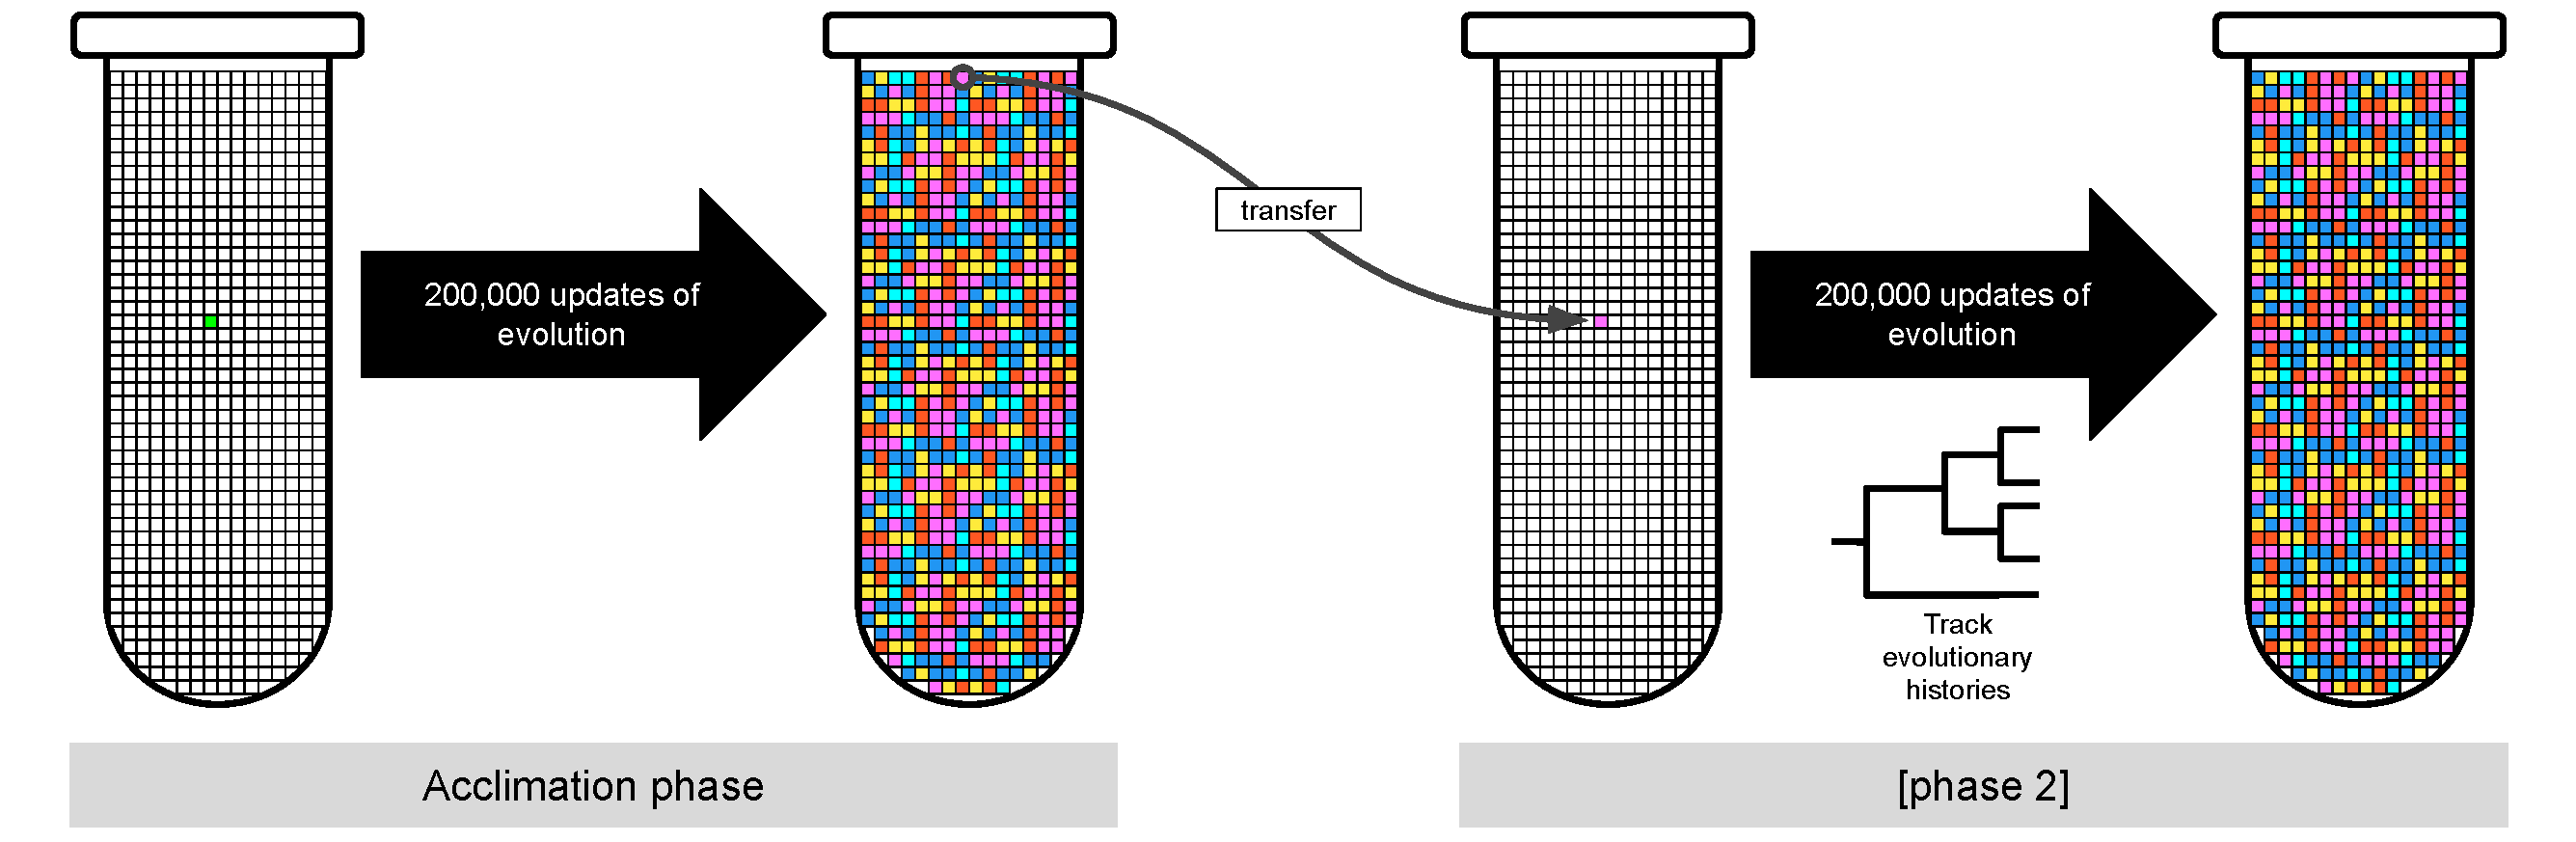
\includegraphics[width=\textwidth]{media/experiment-overview-draft.pdf}
    \caption{\small
    \textbf{todo.}
    todo.
    }
    \label{fig:experimental-design-overview}
\end{figure}

In each experiment described below, we conducted 100 replicates each of three treatments:
\begin{enumerate}
    \item PLASTIC: the environment fluctuates between ENV-A and ENV-B, and digital organisms can differentiate between ENV-A and ENV-B using sensory instructions. As such, adaptive plasticity can evolve.
    \item NON-PLASTIC: the environment fluctuations between ENV-A and ENV-B, but sensory instructions are disabled. As such, plasticity cannot evolve.
    \item STATIC: a control where organisms evolve in a constant environment (ENV-ALL), and thus sensors provide no information.
\end{enumerate}

In both the PLASTIC and NON-PLASTIC conditions, the environment cycles between equal-length periods of ENV-A and ENV-B.
Each of these periods persist for 100 updates (approximately 15 to 20 generations); thus, populations experience a total of 1,000 full periods of ENV-A and 1,000 full periods of ENV-B during each phase.

Phase one gives populations time to adapt to their treatment conditions, affording adaptive phenotypic plasticity the opportunity to evolve \textit{de novo} in the PLASTIC treatment.
At the end of phase one, we extract the most abundant (i.e., dominant) genotype from each replicate population to seed a new population for phase two.
The evolution of optimal phenotypic plasticity is not a guaranteed outcome in the PLASTIC treatment; for this condition, we only continue to phase two if the dominant genotype perfectly regulates which tasks it performs in ENV-A and ENV-B.
This ensures that measurements taken during the experimental phase of the PLASTIC treatment are representative of populations with adaptive phenotypic plasticity.

\vspace{1cm}
\subsubsection{Metrics for quantifying the tape of life}
\label{sec:methods:measurements}
% @AML: Like the idea of an even more general heading. Some ideas:
%  - Measurements
%  - Measuring evolutionary change
%  - Measuring evolutionary history
%  - Measuring evolutionary dynamics
%  - Quantifying the tape of life (call out to the quantifying tape of life paper!)
%  - Quantifying evolutionary change

We analyzed the effects of phenotypic plasticity on evolutionary dynamics by quantifying the evolutionary histories of evolving populations.
Specifically, we examined four metrics (the first three are reviewed in \citep{dolson_interpreting_2020}):
(1) number of coalescence events that have occurred, which indicates the frequency of selective sweeps in the population;
(2) mutation accumulation, which is the sum of all mutations that have occurred along a lineage;
(3) phenotypic volatility, which counts the instances that parent and offspring phenotypes do not match along a lineage, as measured under a given condition;
and (4) mutational stability, which is the fraction of \textit{mutated} offspring long a lineage whose phenotypes do not match that of their parent, as measured under a given condition.

% --- Coalescence/Selective sweeps ---
% Phylogenies should coalesce periodically in asexual populations without ecolocial interactions fostering coexistence.
In asexual populations without ecological interactions fostering coexistence, phylogenies should coalesce periodically; that is, the most recent common ancestor shared by the extant population should change.
The rate that these coalescence events occur can indicate the strength of selection.
For example, populations under strong selective pressures should experience more rapid coalescence events than populations under weaker selection \citep{dolson_interpreting_2020}.

% [Sentence about when we might expect *frequent* selective sweeps].
% We track the rate of coalescence events: how often the most recent common ancestor for each evolving population changes.
% [todo - more literature review on coalescence theory here].
% [one more sentence tying selective sweeps to rate of evolutionary change with evolutionary theory].

% --- Lineages ---
A complete lineage describes a continuous line of descent, specifying an unbroken chain of parent-offspring relationships.
For phase two of each experimental replicate, we isolated a representative lineage from its seed organism to a member of the dominant genotype at the end of its evolution.
Because our experimental treatments do not support long-term coexistence, each of these lineages represents the majority of evolutionary history from a given population at the end of our experiment.

% @AML: something about how measurement deviations among experimental treatments represent differences in dynamics/selection pressures experienced by populations over time?

% Deviations in measurements taken along lineages from different  
% Deviations among experimental treatments in represent differences in selection pressures/evolutionary dynamics.
% We simplified these lineages by collapsing sequential, genetically identical organisms into a single state represented by the associated genotype.
% Given the deterministic nature of genome execution, such a simplification should not lose any information relevant to this study [cite - supplement].

% -- Mutation accumulation ---
Mutation accumulation measures the total number of mutations along a lineage \citep{dolson_interpreting_2020}.
For example, a genotype on the lineage that is two substitution mutations and one insertion mutation away from its parent genotype increases mutation accumulation by three.
Note that for this measure of mutation accumulation, we do not distinguish between beneficial, neutral, or deleterious mutations. 
Instead, we use mutation accumulation as a measure of \textit{overall} genomic change.

% Different evolutionary contexts are expected to result in different rates of mutation accumulation along successful lineages [citations; Barrick 2013?].
% Most trivially, we expect larger mutation accumulation in environments with high mutation rates.
% We would expect strong [purifying/stabilizing] selection to result in lower mutation accumulation relative to lineages evolved under weak selection with [large amount of genetic drift] [citations].
% We might also expect lineages that must continuously adapt to a changing environment via \textit{de novo} genetic changes to exhibit high mutation accumulation relative to lineages evolved under constant environmental conditions [citations; Tape of life].

% -- Phenotypic volatility --
We measure phenotypic volatility as the sum of mutationally-induced phenotypic changes observed along a lineage under a given condition \citep{dolson_interpreting_2020}.
To calculate phenotypic volatility for a given lineage, we express (i.e., evaluate) each genotype along that lineage in a treatment-specific condition, and we sum the number of changes in task profiles between consecutive genotypes.
For lineages evolved in environments fluctuating between ENV-A and ENV-B, we evaluate genotypes in both environmental conditions and count only changes in its \textit{aggregate} phenotype; this technique ensures that environmentally-induced changes are excluded from our measurement.
This phenotypic volatility metric illuminates the rate at which accumulated genetic changes actually change the phenotype along a lineage. % @AML: need better language to talk about 'comprehensive/full' phenotype

% -- Mutational stability --
We measured mutational stability as the fraction of mutated offspring along a given lineage with a different phenotype than their parent.
For lineages evolved in fluctuating environments, we evaluated mutants under both ENV-A and ENV-B and counted all changes in the \textit{aggregate} task profile; like our measure of phenotypic volatility, this technique ensures that environmentally-induced changes are excluded from our measurement.
Mutational stability examines the frequency at which mutations effect changes in an offspring's phenotype.

\vspace{1cm}
\subsubsection{Experiment I: Does adaptive phenotypic plasticity constrain evolutionary change?}
\label{sec:methods:experiment-evolutionary-dynamics}

In our first experiment, we examined how the evolution of adaptive plasticity affects the rate of subsequent evolutionary change in fluctuating environments.
Specifically, we examined the four metrics (described above) across PLASTIC, NON-PLASTIC, and STATIC treatments:
(1) number of coalescence events,
(2) mutation accumulation,
(3) phenotypic volatility,
and (4) mutational stability.

% -- genetic architecture analysis --
% How does this tie to genetic architecture, and why would that affect rates of change?
To investigate \textit{why} phenotypic plasticity might alter the rate of evolutionary change, we examine the genetic architecture of organisms evolved under each condition.
While Avida clearly defines the mechanics of each instruction, the emergent function of an instruction depends on its context within a genome. 
For an individual organism, we can perform knockout experiments to identify which instructions are responsible for producing a given phenotypic outcome.

To perform a knockout, we duplicate the organism, replacing a single instruction with an inert ``no-operation'' instruction.
We then identify any phenotypic changes by contrasting the execution results of the ``knockout'' organism and the original.
Such changes provide evidence of the role that the original instruction must have played in the genome.
For example, when an organism performs the NAND task but loses it when an instruction is knocked out, we categorize that instruction as part of the NAND task machinery.
We use knockout experiments to characterize the role of each instruction in the genomes of every organism along all study lineages, revealing how genetic architectures change over time.
[specifically, we compared x, y, and z...].

\vspace{0.5cm}
\subsubsection{Experiment II: Does adaptive phenotypic plasticity promote the subsequent evolution of novel traits?}
\label{sec:methods:experiment-novel-traits}

% -- overview --
We tested how the evolution of adaptive phenotypic plasticity influences the potential for novel adaptive traits to evolve.
In this experiment (across all treatments), we used the expanded task set of 77 Boolean logic tasks during the second phase of evolution \citep{ofria_avida:_2009}.
This task set includes the six phase one tasks (NOT, NAND, AND, OR-NOT, OR, and AND-NOT; hereafter called ``base'' tasks) plus 71 new phase two tasks (hereafter called ``novel'' tasks).
Across all experimental treatments, organisms could improve their metabolic rate by performing any of the 71 novel tasks.
The six base tasks were still present in the environment and continued to be rewarded or punished according to the particular treatment.
% @AML: line below is cut-able if necessary
As such, in fluctuating environments, the six base tasks continued to fluctuate, but the additional 71 tasks were always rewarded; in static environments, performing any of the 77 logic tasks was always beneficial.

% --additional tasks--
An organism receives a \novelTraitsReward\ metabolic rate improvement for each of the novel tasks that it performs (limited to one reward per unique task).
This reward provides a selective pressure to evolve these tasks, but their benefits do not overwhelm existing treatment-specific selective pressures.
As such, populations in the PLASTIC and NON-PLASTIC treatments cannot easily escape environmental fluctuations by abandoning the fluctuating base tasks.
% Performing a fluctuating task in the appropriate environment ([a,b,c] in ENV-A and [x,y,z] in ENV-B) results in a two-fold metabolic rate improvement, whereas, at a \novelTraitsReward\ reward rate, 8 additional tasks are equivalent single rewarded fluctuating task; further, the majority of the 71 additional tasks require more complex genetic machinery to perform than the six fluctuating tasks.

% - performance evaluation -
We measured task discovery, task performance, and task loss along successful lineages to examine the extent to which populations are capable of acquiring and retaining novel traits. % are more or less evolvable
We limited these measures to the novel task set, excluding the six base tasks:

\begin{itemize}
    \item \textbf{Task discovery} measures a given lineage's level of \textit{exploration} of the fitness landscape [cite - Rose].
We calculated task discovery as the total number of unique tasks ever performed along the lineage, even if a task is later lost; as such, a lineage's task discovery measurement could range from 0 to 71.

\item \textbf{Task performance} measures the level of \textit{exploitation} of the fitness landscape at a given point in time.
In this work, we summarized task performance using a count of unique tasks completed by a representative organism from each population.
We focused on an organism from the dominant genotype at the end of the experiment as the most representative phenotype in the evolved population.

\item \textbf{Task loss} measures how often a lineage fails to retain evolved traits over time and thus indicates the ability for traits to be maintained over time.
We calculated task loss as the number of times along a lineage that a task is performed by a parent but not its offspring. 

\end{itemize}

\vspace{0.5cm}
\subsubsection{Experiment III: Does adaptive phenotypic plasticity decrease deleterious hitchhiking?}
\label{sec:methods:experiment-deleterious-hitchhiking}

Given that preliminary experiments showed numerous deleterious mutations, we conducted tests to determine the role of genetic hitchhiking in these results.
In asexual populations without horizontal gene transfer, all mutations are linked.
As such, deleterious mutations that co-occur with a beneficial mutation can sometimes `hitchhike' to fixation \citep{smith_hitch-hiking_1974,van_den_bergh_experimental_2018}.
Without such co-occurrence, natural selection normally prevents deleterious mutations from reaching high frequencies. 
However, hitchhiking effects have been shown to drive deleterious mutations to high frequencies \citep{buskirk_hitchhiking_2017}. %[citations]. 

To test each of the PLASTIC, NON-PLASTIC, and STATIC treatment's susceptibility to hitchhiking, we added a \code{poison} instruction to the instruction set during the second phase of this experiment.
When executed by an organism, the \code{poison} instruction reduces the organism's metabolic rate (and thus reproductive success), but does not otherwise alter the organism's function.
Here, we imposed a 10\% penalty each time an organism executed this instruction, making the instruct explicitly deleterious (see [supplementary material] for tests with 3\% and 30\% penalties, which produced consistent experimental results).

% - measurements -
At the beginning of phase two, the \code{poison} instruction is not present in the population as it was not part of the instruction set during the first phase of evolution.
However, by adding \code{poison} to the instruction set during phase two, it can be introduced via a mutation.
We measured susceptibility to genetic hitchhiking by examining the number of times a \code{poison} instruction is executed by each genotype along the dominant lineage (including the final dominant genotype).
Because the \code{poison} instruction is explicitly deleterious, we expect it to show up in successful lineages only as a result of hitchhiking, as selection should purge deleterious mutations not linked to beneficial mutations.

\vspace{0.5cm}
\subsection{Data analysis and software availability}

Across all of our experiments, we differentiated between sample distributions using non-parametric statistical tests.
For each major analysis, we first performed a Kruskal-Wallis test \citep{kruskal_use_1952} to 
determine if there were significant differences in results from the PLASTIC, NON-PLASTIC, and STATIC treatments.
If so, we applied a Wilcoxon rank-sum test \citep{kotz_individual_1992} to distinguish between pairs of treatments.
We applied Bonferroni corrections for multiple comparisons \citep{rice_analyzing_1989} where appropriate.

We conducted our experiments using a modified version of the Avida software, which is open source and freely available on GitHub [cite].
We used Python [cite] for data processing, and we conducted all statistical analyses using R version [x] [cite].
We used the tidyverse collection of R packages [cite] to wrangle data, and we used the following R packages for graphing and visualization: [list and citations].
We used R markdown [cite] and bookdown [cite] to generate web-enabled supplemental material.
All of the source code for our experiments and analyses, including guides for replication and configuration files, can be found in our supplemental material [cite].
Additionally, our experimental data is available on the Open Science framework at [url] [cite].